\section{Automated embedded field selection}
PeerDB lets you embed fields to obtain faster reads on those fields at the expense of more time for writes and higher network traffic. 
For the benchmarks, we manually selected which fields to embed for the post document. 
Here we present a general algorithm for picking fields to embed in document based on the expected impact of embedding vs referencing a set of fields under a given workload.

\subsection{Overview}
Our algorithm optimizes the configuration of embedded fields in a main document $D$ according to a workload specification. 
For instance, if a post document $D$ references an author document, we could choose to embed all of the author's fields, none of the authors fields or some combination of these options. 
To choose between many possible configurations, our algorithm takes into account the expected field read and field write workloads specified by the user along with expected field size. 
Then, the algorithm assigns a cost to each configuration based on an approximate cost model. The algorithm returns the user the lowest cost configuration. 
The user uses this configuration to specify which fields to embed under their expected workload.

\subsection{Workload specification}
For queries to a given document, $D$, users need to supply how often they will query each all document fields and fields in related documents $D_R$. 
Specifically, for all fields $f_i \in D, D_R$ users specify, an expected frequency of reads originating from $D$ for each field, $E_R(f_i)$, an expected frequency of writes for each field, $E_W(f_i)$, and an expected size of each field $E_S(f_i)$. 

\subsection{Cost model}
Our cost model assigns a cost to a document configuration $C =$\{$c_1, c_2, ... c_n | c_i = 1 \text{ if field } f_i \in D_R \text{ is embedded }$\} considering expected read time, $R$, write time $W$, and traffic $T$ under a given workload specification, $S$.
$$Cost(C,S) = w_R*R + w_W*W + w_T*T$$ 
The parameters $w_R$ and $w_W$ allow the user to set the importance of the read-time and write-time respectively. 
For instance, the user may set the $w_R$ higher than $w_W$ in the case that website visitors read documents, but only admins write documents. 
As we do not consider the network traffic of calls other than those for the given document and it's fields, $w_T$ can be used to adjust the importance of keeping the number of messages passed as a result of document calls to a minimum.

\subsubsection{Computing read-time term, $R$}
The read-time term takes into account the read-times for all document fields and referenced document fields in a given configuration, $C$, for a given workload, $S$. 
$F$ means all fields $f_i$. 
We define $F_0$ as all fields $f_i$ where $c_i = 0$ and $F_1$ as all fields $f_i$ where $c_i = 1$. $F_D$ encompasses all fields in the base document which are not assigned in the configuration. 
The equation for $R$ also takes into account the time to request data, $M$, and the time to read one KB of data $K$:
\begin{align*}
R =& [M + max(E_R(f_i) \forall f_i \in F_1 \cup F_D)*\sum_{f_i \in F_1 \cup F_D} K*E_S(f_i)\\
& + \sum_{D_{R_i} \in D_R} \{M + max(E_R(f_i) \forall f_i \in D_{R_i} \cap F_0)\\
& * \sum_{f_i \in D_{R_i} \cap F_0} K*E_S(f_i)\} + P]
\end{align*}
The first summation calculates the expected read time for all document fields ($F_D$) and embedded fields ($F_1$). 
The second summation adds the expected read time for all secondary requests for referrenced documents and all time required to read the fields ($F_0$) of those documents. 
Because we assume we read all data from each document when we fetch it, the $max$ terms calculate how many times we need to fetch each document to match the required field reads. 
Overall, this equation shows that embedding a field saves read time for secondary requests incurred by referenced documents and their fields. 
We can see that embedding fields will decrease read-time in cases where the cost of a secondary request is high, or where the referenced documents are large.

Finally, $P$ is the penalty for inconsistency. 
If a read occurs before the write data is consistent, the read must recursively reference the referred document. 
$P$ accounts for the additional time for reacursively referencing the referred document as it was not covered in the other summations. 
For each embedded document, we add back on the time to retrieve the referenced document multiplied by the chance that the field is read while the data is in consistent, $I(f_i)$, which depends the frequency of writes and reads. 
Here $D_{R_{F_1}}$ refers to all documents that have an embedded field. 
$$P = I*\sum_{D_{R_i} \in D_{R_{F_1}}} [M+\sum_{f_i \in D_{R_i}} K*E_S(f_i)*E_R(f_i)]$$
In our implementation we set $I(f_i) = 0 \forall f_i \in F$. 
In future work, we will use detailed analysis to figure out how to relate the frequency of writes and reads to the chance that the read data is inconsistent. 
Like $M$ and $K$, this term will be unique to each system.

\subsubsection{Computing the write-time term $W$}
The write-time term takes into account the write times for all $f_i \in D, D_R$ for a given configuration $C$ and workload $S$. 
\begin{align*}
W =& [\sum_{f_i \in F_1} K*E_S(f_i)*E_W(f_i)\\
& + \sum_{f_i \in F} K*E_S(f_i)*E_W(f_i)]
\end{align*}
The first summation counts time for embedded fields, and the second summation counts time for all fields. This means embedded fields require two writes to update the referenced document whereas referenced documents only require one write. 
The write-time term $W$ displays that embedding fields will not be beneficial in write-heavy workloads.

\subsubsection{Computing the traffic term, $T$}
We add the term $T$ with its weight $w_T$ to allow the user to adjust how important it is to keep the network traffic from PeerDB low. 
$T$ is the number of messages passed based on reads and writes. 
\begin{align*}
T=& 2*|D\text{ reads}| + 2*|D_R\text{ reads}|\\
& + 4*|\text{embedded writes}| + 2*|\text{referenced writes}| 
\end{align*}

\subsection{Picking a configuration}
The total number of possible configurations for any schema is $2^n$ where $n$ represents the number of fields in referenced documents. 
In our implemnentation, $n$ is small so we use a brute force approach to find the configuration with the lowest cost. 
In cases where $n$ is large, we could apply a greedy algorithm or simulated annealing to find a near-optimal answer.

\subsection{Evaluation}
We implemented our model and tested it on one schema (Figure~\ref{fig:schema}) under several different workload specifications and parameter weightings. 

First, we ran our algorithm with the illustrated schema (Figure~\ref{fig:schema}) and workload specification (Table~\ref{workload}) with the parameter settings $w_R = 1, w_W = 0, w_T = 0$. Under these settings, the algorithm tells us that the lowest cost configuration embeds the author name and tag name, but no other fields. 
This is not surprising: only considering the read-time term, we expect fields often read with post that are not large to be embedded. 
The author picture field is large and only occasionally read with $D$.
As a result, the algorithm does not embed the author picture to avoid fetching it on every post query.

Setting the parameters to $w_R = 0, w_W = 1, w_T = 0$ (only considering writes), the algorithm tells us to not embed any fields, because every embedded field incurs extra write time.
Finally, setting the parameters to only pay attention to the messages passed, $w_R = 0, w_W = 0, w_T = 1$ we get that we should embed all fields except author bio and tag description. 
The algorithm picks this configuration because we provided a read-heavy workload, and each non-embedded field requires extra messages to read. 

For this schema and workload, if we set the parameters to $w_R = 1, w_W = 1, w_T = 0$ we unsurprisingly get the same configuration as suggested by considering the read time alone. 
However, if we switch the expected read values in the workload specification with the expected write values in the specification and leave the parameters as  $w_R = 1, w_W = 1, w_T = 0$, the algorithm tells us to not embed any fields. 

Overall, our algorithm agrees with intuition in these cases. Such an algorithm can pick the lowest cost fields to embed based on a schema and an expected workload specification.

\subsection{Implementation}
This algorithm was implemented in unoptimized Python code on a MacBook Pro. Each run of the algorithm to consider all embeddings and return the lowest cost configuration took around ~2ms.

\begin{figure}[t]
\centering
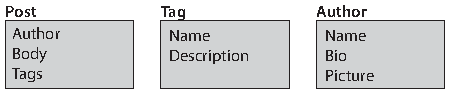
\includegraphics[width=3.33in]{figures/algorithm-schema.pdf}
\caption{We tested our algorithm with a schema where post was the main document $D$, and the post referenced related documents author and tags. All possible configurations of post are embedding all related document fields, none of the related document fields, or any combinations of the related document fields.}
\label{fig:schema}
\end{figure}


\begin{table}
  \small
  \begin{center}
  \begin{tabular}{|l|l|l|l|}
    %\hline
    \hline
    Field & $E_S$ (KB) & $E_R$ (reads/day) & $E_W$ (writes/day)\\ \hline
    Author name & .1 & 1000 & 1 \\
    Author bio & 1 & 0 & 5 \\ 
    Author picture & 1000 & 50 & 5 \\ 
    Tag name & .1 & 1000 & 1 \\ 
    Tag description & 1 & 0 & 2 \\ 
    Post body & 10 & 1000 & 1 \\ \hline

  \end{tabular}
  \end{center}
  \caption{Here is a sample workload specification for our schema. We quantify expected reads and writes per day over fields from all post documents. In this case, we have a read-heavy workload where most views include the author name, post body, and tag names with the post, but only some views include the author picture.}
  \label{workload}
  \vspace{-4mm}
\end{table}

In future work we will rigorously test our model to make sure it matches the benchmark expectations. 

\subsection{Discussion}
Although useful for many applications, our model makes several simplifications. 
For instance, our model does not take into account the reverse field feature of PeerDB. 
Further, our model does not take into account the possibility of embedding an entire referenced document instead of using PeerDB. 
Embedding without PeerDB the document instead of providing a reference is helpful in cases where you only reference the embedded document from the parent document~\cite{MongoDB2014}. 
In the future, we will add this option by augmenting the model and workload specification to include querying documents aside from the main document $D$. 
Our model also assumes that you read all information in a document when you fetch it. 
In the future we could let the user specify which combinations of fields they would read and adjust our cost model to handle such specifications.

We also made other minor simplifications, such as using the same constants $K$ and $M$ for all writes and reads. 
In reality, these numbers are different for writes and reads. 
In the future, we could provide an application to learn these constants for any given system. 
